\chapter{Risultati}
Per poter definire l'efficienza e l'effettiva scalabilità del sistema creato 
è necessario misurare le sue prestazioni. 
A questo fine, vengono eseguiti dei test che effettuano un elevato numero di richieste,
per valutare il suo comportamento in momenti di grande utilizzo e
verificare così che sia garantita la qualità del servizio, anche in situazioni di stress.\\
\\
Nell'ottica di ottenere dei risultati che descrivano fedelmente 
il comportamento dell'applicazione, 
evitando però di eseguire un test su ogni funzione implementata,
sono state selezionate alcune funzionalità.
La scelta di queste funzionalità deriva dalla capacità 
di poter ricondurre le loro prestazioni a tutto il resto del sistema,
in base sia alla similitudine nel comportamento,
che all'utilizzo dei vari servizi, che permette di misurarne la qualità della cooperazione.\\
\\
In particolare, le funzionalità di creazione e selezione degli eventi permettono 
di valutare direttamente le prestazioni in scrittura e lettura dei dati sul database, 
influenzando Azure Functions e Cosmos.
L'aggiornamento di un dato di un evento,
richiedendo una scrittura parziale, 
consente di misurare anche questa particolarità dei database non relazionali.
Ancora più rilevanti però sono le conseguenze che scatena.
Per garantire la consistenza la funzione aggiunge infatti un messaggio in coda al Service Bus,
che verrà poi preso in carico da un'altra Azure Function.
Infine, la richiesta di caricamento delle immagini ci permette 
di valutare il rapporto con Azure Storage Container, 
ultimo componente fondamentale dell'applicazione.
\clearpage
\section{Impostazione dei test}

Per l'implementazione dei test è stato usato Azure Load Testing.
Azure Load Testing(ALT) è un servizio che dà la possibilità
di eseguire delle richieste secondo un carico impostabile,
\begin{wrapfigure}{o}{0.25\textwidth}
    \centering
    
\includegraphics[height=.12\textheight]{loadtest.png}
    Azure Load Testing
\end{wrapfigure}
per poi monitorarne e mostrarne i risultati.
Questo permette di testare le prestazioni dei servizi direttamente all'interno della piattaforma.
Integrandosi con l'ambiente Azure
consente inoltre di associare al test il monitoraggio di ulteriori risorse,  
allineando ai risultati complessivi le prestazioni riportate dai singoli componenti, 
permettendo analisi più comprensive e puntuali.\\
\\
Il carico viene definito tramite diversi parametri che possono essere impostati 
attraverso l'interfaccia o in un file di configurazione.
Vengono così stabiliti la durata del test, il numero di istanze (ovvero server fisici su cui verrà eseguito il test)
e il numero di thread per istanza.
Per thread si intente un processo che, in parallelo con gli altri, 
esegue le richieste, 
fornendo un'idea generale sulla quantità delle richieste che verranno create.
Se le istanze sono più di una,
si può decidere di distribuirle su server in diverse posizioni geografiche,
per ottenere informazioni relative alla qualità del servizio in diverse parti del globo.\\
\\
Azure presenta tre modalità secondo le quali il carico può variare: 
lineare, in cui il carico varia stabilmente, 
scalare, nel quale il carico aumenta ogni intervallo di una quantità stabilita e
picco, in cui il carico viene concentrato in un breve intervallo di tempo.
Una volta stabilita la modalità, sarà necessario definire le caratteristiche 
che descrivono il suo comportamento. 
Ad esempio, la modalità lineare necessita di sapere in quanto tempo arrivare al carico massimo.
In ogni caso è richiesta la durata del test.\\
\\
I test possono essere eseguiti tramite url o usando un file di configurazione.
Il primo caso necessita che la funzione da testare risponda a una richiesta HTTP.
Il test prevede semplicemente la sua invocazione per il numero desiderato di volte.
Permette di essere configurata completamente tramite interfaccia grafica,
e risponde alla maggioranza delle necessità per testare prestazioni generiche.
Nel caso in cui si voglia però misurare funzionalità più complesse, 
che richiedono l'interazione con file esterni, la modifica in corso delle richieste o 
l'esecuzione di più richieste in successione, è necessario utilizzare un file apposito.\\
\\
All'interno del file di configurazione bisogna indicare, tramite un apposito codice,
il carico voluto e le richieste da eseguire.
Oltre a fornire una maggiore precisione nella definizione del carico, 
la possibilità di impostare la modalità del test
consente un'elevata libertà nel stabilire le proprietà delle richieste e le loro eventuali interazioni.
Questo permette, ad esempio, di caricare e leggere file, 
che possono contenere informazioni utili per variare le richieste o
possono essere usati per scambiare dati.
Si può inoltre simulare un'interazione più complessa,
in cui si aspetta una richiesta per ricevere il risultato, 
per poi usarlo per inviarne una seconda.\\
\\
Il file può essere sviluppato usando Apache JMeter o Locust come codici di configurazione.
I test sono stati implementati in JMeter,
essendo quello utilizzato di default da Azure.
L'interfaccia di Azure Load Testing per la creazione del test tramite del file di configurazione
prevede il suo inserimento, assieme a tutti gli eventuali file allegati di cui necessita.
Prevede inoltre l'impostazione del numero di istanze 
per il quale si vuole distribuire il test, nelle quali verrà duplicato.\\
\\
Per ogni test di entrambe le modalità si possono infine specificare quali altre risorse del progetto monitorare,
affiancando alle prestazioni generali del test le prestazioni specifiche dei singoli componenti.

\section{Velocità della procedura di creazione}

Il primo test si concentra sulla velocità di creazione di elementi.
La creazione è un'operazione che richiede l'inizializzazione logica di oggetti in un'Azure function, 
per poi procedere a salvarli sul database.
Per quanto l'interazione logica comporti un tempo limitato, 
il salvataggio dei dati sul database è un'azione che richiede normalmente tempi significativi, 
in quanto comporta la scrittura diretta sul disco.\\
\\
In particolare, si è scelto di testare la creazione di un nuovo evento,
vista sia la sua centralità nell'applicazione che la sua complessità logica.
La creazione di un nuovo evento infatti comporta, 
oltre alla creazione dell'elemento Event stesso,
l'inizializzazione dei ProfileEvent ed EventProfile associati.
Il loro salvataggio avviene in seguito alla creazione dell'oggetto Event,
per cui è introdotta una logica transazionale che garantisce l'atomicità della richiesta.
L'esecuzione di questo test consente quindi di analizzare la capacità del sistema 
nel ricevere ed eseguire scritture complesse sul database, 
senza il coinvolgimento di ulteriori risorse.\\
\\
La funzione di creazione di un evento è semplice,
richiedendo un solo passaggio e presentando dei dati in ingresso che possono essere prestabiliti.
Viene quindi usato un test che invoca la funzione tramite url,
con un carico di richieste della durata di due minuti, 
che aumenta linearmente nei primi trenta secondi per poi stabilizzarsi.
Questo permette di analizzare il sistema sia in base al numero di richieste in contemporanea,
che durante un periodo di richieste alto ma costante.
Al test vengono affiancate le metriche delle Azure Functions, 
monitorate attraverso le Application Insights,
per misurare i risultati lato server,
assieme a quelle del database Cosmos, 
per determinare con più facilità la causa di eventuali errori.\\
\begin{figure}[htbp]
    \begin{center}
        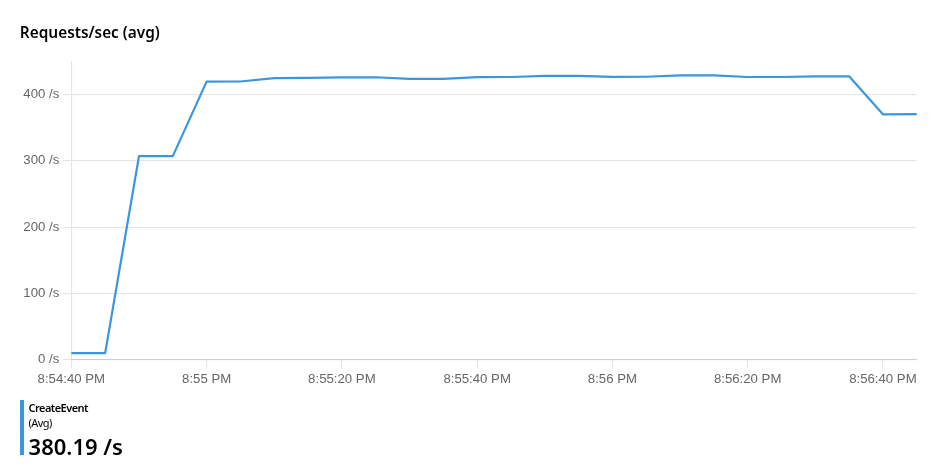
\includegraphics[width=\textwidth]{create_load.png}
        \caption{Carico delle richieste per la creazione di eventi}
    \end{center}
\end{figure}\\

Il test così creato ha portato alla creazione di 49425 Event
nell'arco di due minuti, sostenendo con successo un carico di, mediamente,
386 richieste al secondo.
Tutte le richieste sono andate a buon fine, con un tempo di risposta di 243 ms.
Questa durata è però comprensiva del tempo di trasmissione dei dati.
Analizzando i dati registrati da Application Insights,
si nota che il tempo medio delle richieste si abbassa a 133 ms.\\
\begin{figure}[htbp]
    \begin{center}
        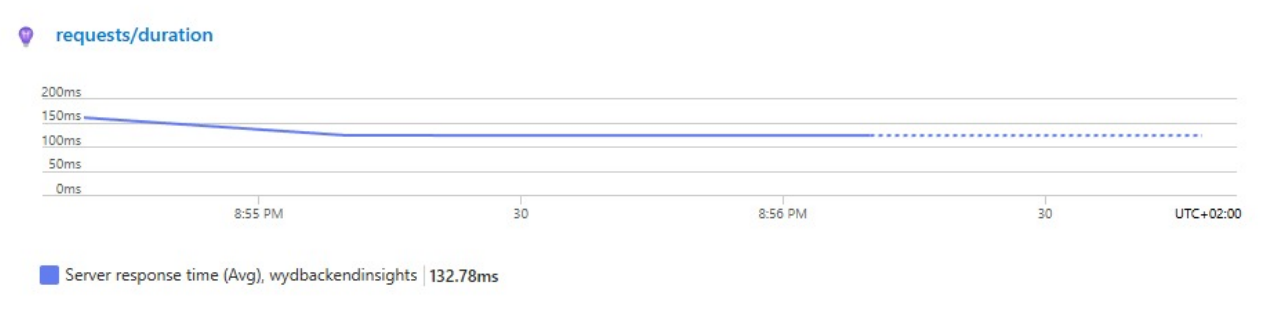
\includegraphics[width=\textwidth]{create_server_time.png}
        \caption{Tempo medio delle richieste lato server}
    \end{center}
\end{figure}
\\
Si può quindi affermare che il sistema è in grado di affrontare efficacemente 
richieste di scritture sul database continuate e parallele, anche complesse o multiple,
limitate, per ora solamente dalle risorse dei servizi.
Il tempo maggiore rilevato all'inizio delle richieste è riconducibile al
tempo di avviamento delle risorse, che rimane stabile una volta inizializzato.
\\
\begin{figure}[htbp]
    \begin{center}
        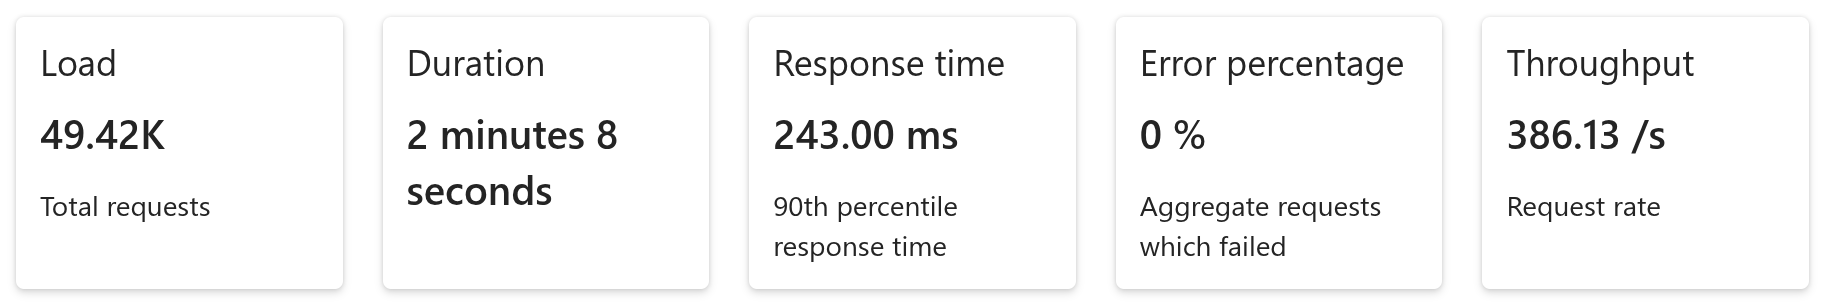
\includegraphics[width=\textwidth]{create_general.png}
        \caption{Risultati del test di creazione}
    \end{center}
\end{figure}
\\
\clearpage

\section{Velocità in lettura}

L'operazione di recupero delle informazioni è centrale 
per fornire all'utente un'esperienza fluida e consistente.
Risulta quindi fondamentale che il tempo di identificazione e lettura dei dati sia il più basso possibile.
Sebbene la scalabilità sia facilitata dalla natura dell'azione,
che può sfruttare copie e può avvenire in contemporanea sullo stesso elemento,
è bene poter garantire che la risposta a operazioni di lettura anche complesse 
non venga degradata in base alla quantità delle richieste.\\
\\
Tra le varie richieste dirette di dati, 
che quindi non comportano aggiornamenti o ulteriori processi,
è stato scelto il recupero degli eventi relativi al profilo corrente.
Questa operazione viene eseguita ogni volta che l'utente chiede dati relativi a un intervallo, 
quando non sono presenti dati in memoria locale.
Oltre a essere importante per il funzionamento generale dell'applicazione,
è anche una delle richieste di lettura più complesse.
Deve infatti recuperare i ProfileEvent relativi al profilo in quell'intervallo,
per poi recuperare gli EventProfile associati da cui poi ricavare l'Event corrispondente.
Per ogni Event così trovato deve poi essere creato un EventDto che contenga 
sia le informazioni dell'Event che di ProfileEvent.
Tutte queste operazioni sono definite in un'Azure Function, 
ma delegate direttamente a Cosmos.
Il numero degli eventi trovati viene limitato a 40.\\
\begin{figure}[htbp]
    \begin{center}
        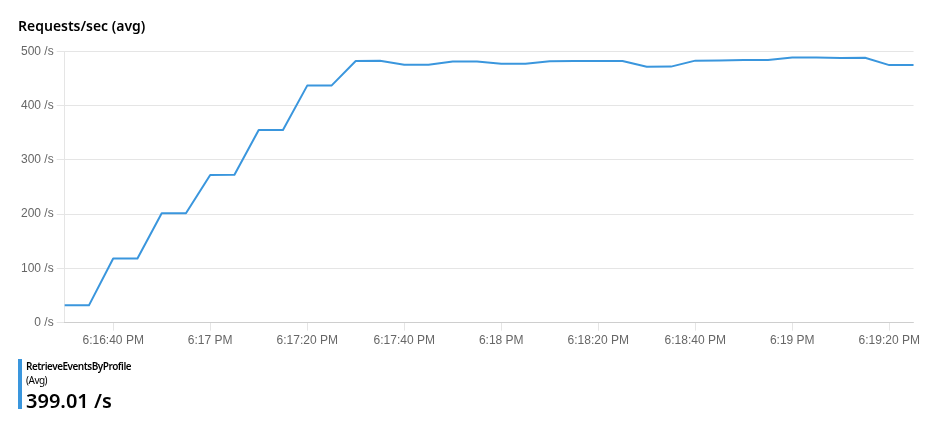
\includegraphics[width=\textwidth]{retrieve_load.png}
        \caption{Carico delle richieste per il recupero di eventi}
    \end{center}
\end{figure}
\\
Anche in questo caso, 
vista la semplicità della richiesta è sufficiente una richiesta tramite url.
Impostato l'identificativo del profilo all'interno della richiesta, 
il test procederà inviando richieste seguendo un carico della durata di tre minuti, 
impiegando i primi trenta secondi a raggiungere linearmente il carico massimo di circa 480 richieste al secondo.
Influenzando solo le Azure Functions e Cosmos, verranno monitorate, come in precedenza, 
solo le Application Insights e Cosmos stesso.\\
\\
Il test ha comportato la lettura di quasi settantunmila richieste,
con una media di quattrocento richieste al secondo.
Non sono stati riscontrati errori.
Il tempo di risposta totale medio è risultato di duecentoquindici millisecondi per richiesta,
che scende però sotto i cento se si considera il tempo di esecuzione effettivamente impiegato dal server.\\
\begin{figure}[htbp]
    \begin{center}
        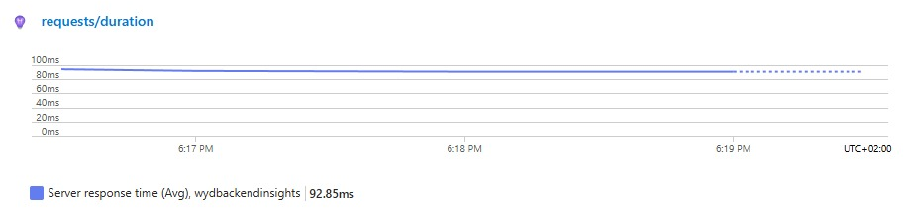
\includegraphics[width=\textwidth]{retrieve_server_time.png}
        \caption{Tempo medio delle richieste lato server}
    \end{center}
\end{figure}
\\
Il successo di questo test conferma le capacità del sistema 
di rispondere a carichi elevati di richieste in lettura contemporanee, 
mantenendo le prestazioni costanti sia in caso di aumento di carico che in caso di richieste frequenti.\\
\begin{figure}[htbp]
    \begin{center}
        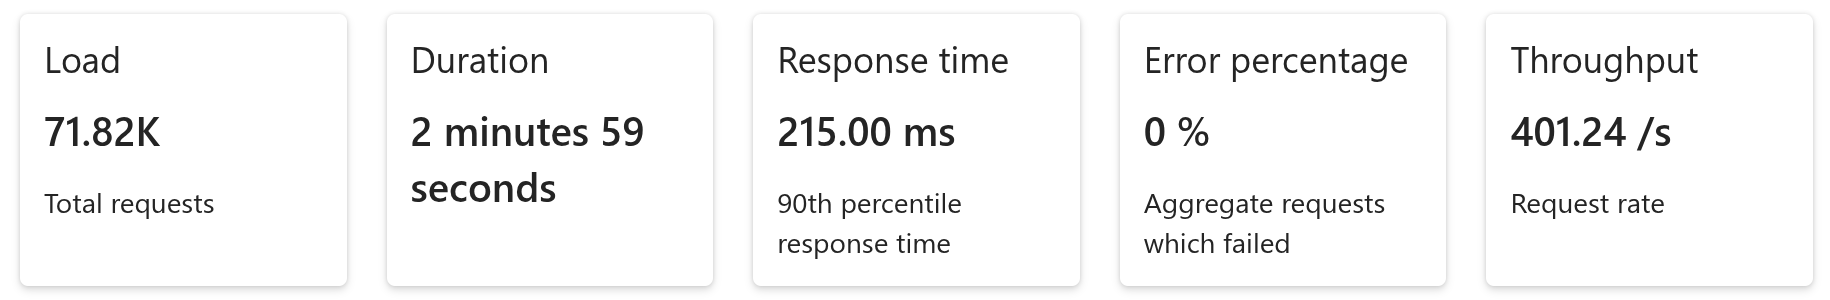
\includegraphics[width=\textwidth]{retrieve_general.png}
        \caption{Risultati del test di creazione}
    \end{center}
\end{figure}
\clearpage

\section{Velocità degli aggiornamenti}
L'aggiornamento di un dato su un database non relazionale
è un'operazione che si distingue dalle precedenti per due principali caratteristiche.
La prima peculiarità consiste nella necessità di ritrovare i dati, 
comportando una ricerca sul database.
La seconda consiste nella possibilità di modificare parti del documento
senza sovrascriverlo completamente.
Per mettere alla prova queste capacità si è deciso di monitorare
le risposte alla modifica di un evento.
Oltre a essere la funzione di aggiornamento probabilmente più richiesta,
permette di testare le prestazioni delle code create per la propagazione delle modifiche.\\
\\
Una volta garantita l'applicazione delle modifiche sull'Event coinvolto, 
la funzione deve inoltre assicurare che queste vengano propagate 
a tutti gli elementi sulle quali sono state denormalizzate le sue informazioni:
in questo caso, tutti i ProfileEvent a esso associati.
I componenti principali coinvolti rimangono Azure Function e Cosmos database,
a cui si aggiunge però Azure Service Bus, 
che prende in carico il messaggio con cui verrà poi eseguita la funzione responsabile 
di sincronizzare le informazioni con le altre entità coinvolte nel database.
La funzione principale dovrà quindi connettersi con il database per effettuare le modifiche,
per poi inviare il messaggio al Service Bus, assicurandosi che sia stato in carico.
Nel caso una di queste due fasi non vada a buon fine, 
l'intera funzione è da considerarsi fallita.\\
\\
La funzione principale risponde a una chiamata HTTP 
per apportare le modifiche richieste con un aggiornamento parziale sul database.
L'impostazione del test tramite url comporterebbe però la convergenza di tutte le richieste
sullo stesso Event, compromettendo l'affidabilità dei risultati,
in quanto rappresentazione di un caso molto particolare quanto improbabile.
Per risolvere questo problema è stato un file JMeter che,
importando da un file l'identificativo dell'Event,
garantisce che le richieste siano distribuite su Event differenti.
Il file allegato contiene tutti gli identificativi degli eventi creati nel primo test,
e il file di configurazione è stato impostato per associare una sola richiesta allo stesso Id.
Questo permette un miglior controllo per i risultati del test successivo.
\clearpage

\begin{figure}[htbp]
    \begin{center}
        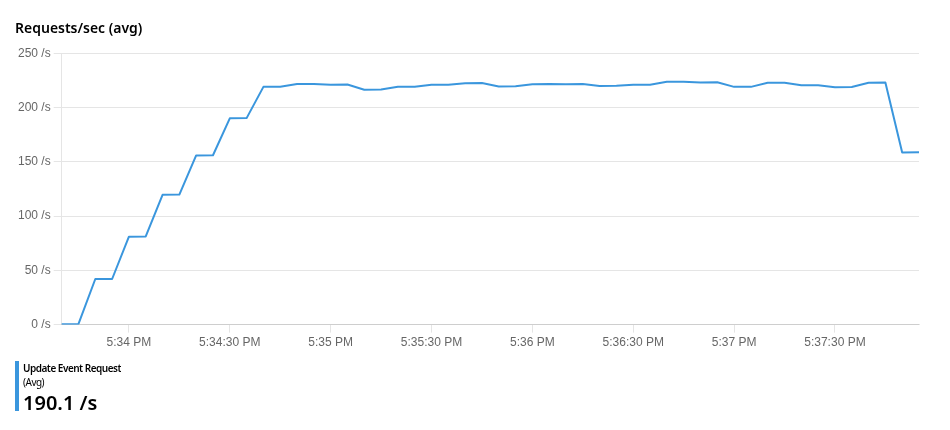
\includegraphics[width=\textwidth]{update_load.png}
        \caption{Carico delle richieste per l'aggiornamento di eventi}
    \end{center}
\end{figure}
La durata del test dipende dal tempo necessario 
per processare tutti gli identificativi presenti sul file allegato.
Come per gli altri casi, si è però deciso di aumentare il carico linearmente per i primi trenta secondi,
per testare sia la risposta in caso di aumento del carico che sotto a stress elevato ma costante.
Al monitoraggio di Application Insigths e di Cosmos
viene aggiunto quello di Service Bus, 
per assicurarsi che effettivamente i messaggi vengano aggiunti alla coda dedicata.\\
\begin{figure}[htbp]
    \begin{center}
        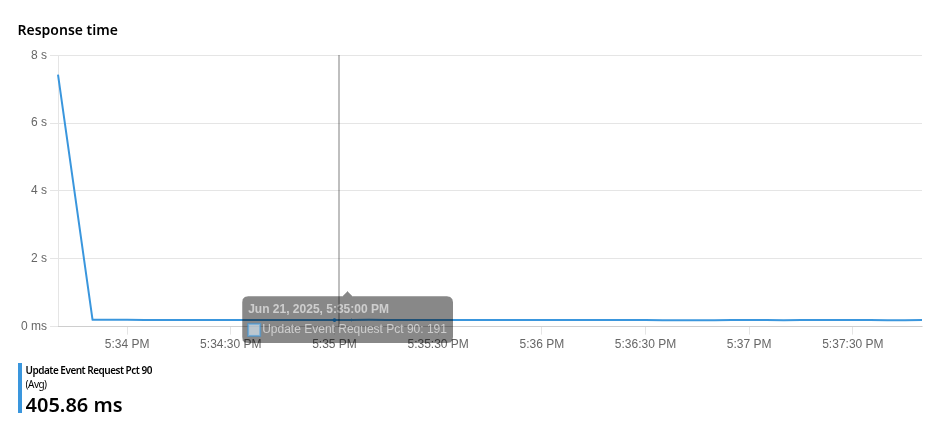
\includegraphics[width=\textwidth]{update_time.png}
        \caption{Durata delle richieste di modifica dell'evento}
    \end{center}
\end{figure}
\\
Il test ha così prodotto un carico medio di duecento richieste al secondo 
distribuite in quattro minuti e mezzo, 
con un picco che si è mantenuto costante negli ultimi tre minuti di duecentoventi richieste al secondo.
Nonostante un tempo iniziale elevato dovuto all'inizializzazione del server, 
che impatta sul tempo medio della risposta, 
il tempo medio totale richiesto per l'esecuzione della richiesta è rimasto costante sui duecento millisecondi,
che includono però anche il tempo di trasmissione dei dati e della risposta.
Tutte le richieste sono andate a buon fine.\\
\begin{figure}[htbp]
    \begin{center}
        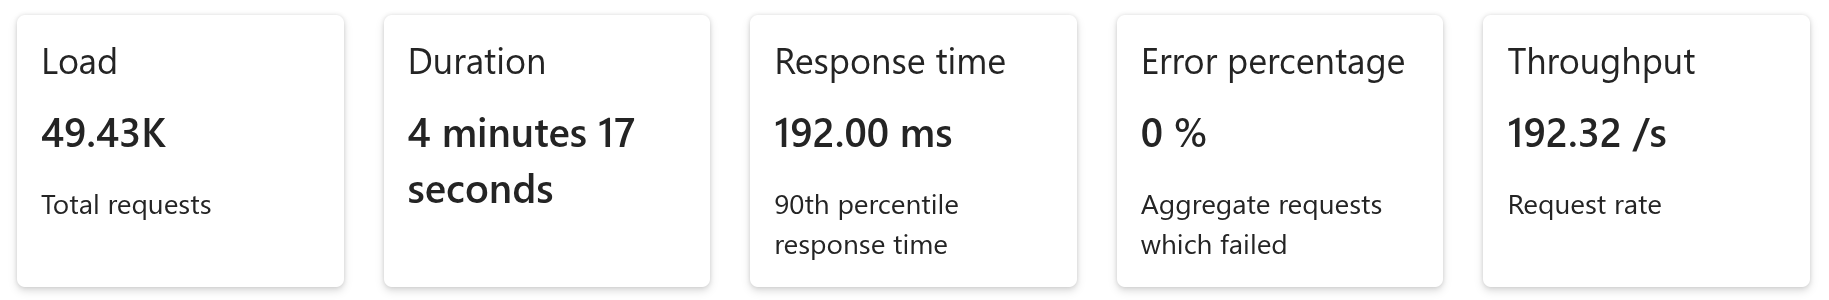
\includegraphics[width=\textwidth]{update_general.png}
        \caption{Risultati del test di aggiornamento}
    \end{center}
\end{figure}
\\
Le prestazioni riscontrate risultano in linea con gli altri risultati,
con un tempo medio di esecuzione effettiva intorno ai centocinquanta millisecondi,
garantendo anche in questo caso un'interazione fluida.
L'aumento o la frequenza della quantità delle richieste non impatta
sul funzionamento o sul ritardo della risposta, 
che rimangono inalterati durante tutta la durata del test.
Il tempo effettivo impiegato dalle Azure Function non è stato analizzato,
in quanto comprensivo della durata delle funzioni che, in contemporanea,
stavano propagando le modifiche sul ProfileEvent.\\

\section{Garanzia di propagazione delle informazioni}

La presenza di elementi denormalizzati comporta la necessità 
di propagare le modifiche sugli elementi coinvolti indirettamente.
Potendo accettare un ritardo tra la modifica dell'elemento principale 
e l'aggiornamento delle sue controparti, 
questo compito viene delegato a un'altra funzione,
riducendo il carico di lavoro (e quindi il tempo di risposta) della prima.
La separazione di questi compiti può essere però sfruttata 
solo se viene garantita l'esecuzione della funzione secondaria incaricata di propagare gli aggiornamenti.\\
\\
Service Bus è stato scelto proprio per la sua proprietà 
di assicurare che il messaggio venga preso in carico da una funzione, 
per poi controllarne l'esecuzione e ripeterla in caso di fallimento.
Dai grafici relativi all'Application Insights si nota una maggiore quantità di esecuzioni, 
così come un tempo medio superiore a quello previsto per l'aggiornamento.
Questo porta a dedurre che le funzioni vengano effettivamente invocate, 
e che il loro tempo di esecuzione sia superiore.\\
\begin{figure}[htbp]
    \begin{center}
        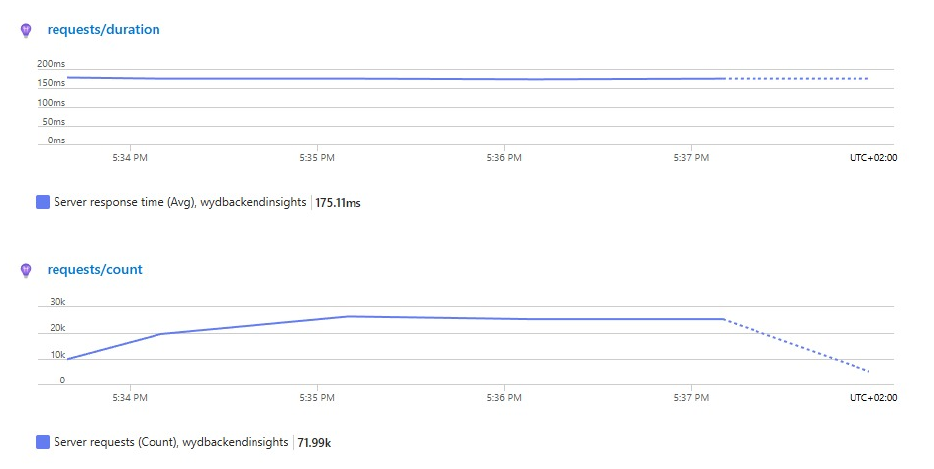
\includegraphics[width=\textwidth]{propagate_server_time.png}
        \caption{Durata e quantità delle Azure Function durante l'aggiornamento}
    \end{center}
\end{figure}
\\
Il monitoraggio di Service Bus conferma ulteriormente la ricezione dei messaggi e 
l'effettiva presa in carico della funzione.\\
\begin{figure}[htbp]
    \begin{center}
        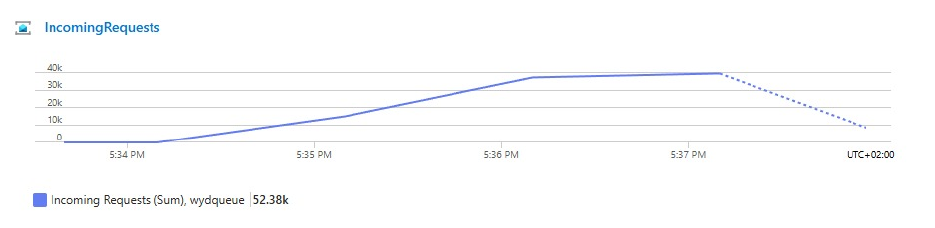
\includegraphics[width=\textwidth]{propagate_servicebus.png}
        \caption{Somma dei messaggi ricevuti da Service Bus}
    \end{center}
\end{figure}
\\
\clearpage
Nonostante la conferma che il collegamento tra Service Bus e Azure Functions
funzioni correttamente in su entrambi i versi, 
è necessario assicurare che gli aggiornamenti siano sempre terminati con successo.
Per controllare che tutti gli aggiornamenti dei ProfileEvent siano andati a buon fine,
il messaggio inviato sul Service Bus che notifica l'aggiornamento dell'Event 
contiene anche il timestamp del momento di attuazione della modifica.\\
\\
La funzione incaricata di allineare i ProfileEvent
salverà quindi, oltre al momento corrente in cui l'aggiornamento avviene,
anche il timestamp dell'aggiornamento dell'Event.
Questo consente, in un secondo tempo, 
sia di certificare che l'aggiornamento sia avvenuto correttamente, 
sia di calcolare il tempo medio che trascorre tra la modifica dell'Event 
e l'effettiva propagazione verso i ProfileEvent.\\
\\
Tramite un programma creato appositamente, 
a termine dell'operazione di aggiornamento degli Event,
sono stati recuperati tutti i ProfileEvent a essi relativi.
Per verificare il successo del processo di propagazione 
è stato controllato che il momento di aggiornamento del ProfileEvent 
fosse successivo a quello dell'Event, 
per poi calcolarne la differenza.\\
\begin{figure}[htbp]
    \begin{center}
        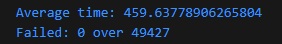
\includegraphics[width=\textwidth]{propagate_results.png}
        \caption{Risultati del programma di controllo sulla propagazione degli aggiornamenti}
    \end{center}
\end{figure}
\\
I risultati del programma hanno successivamente confermato l'affidabilità 
del processo di propagazione dell'aggiornamento tramite Service Bus, 
con un tempo medio di cinquecento millisecondi. 
\clearpage

\section{Velocità di salvataggio delle immagini}
L'ultimo servizio che non è ancora stato testato,
tra i principali che compongono l'applicazione,
è il gestore dei file multimediali: Azure Storage Container.
Azure Storage Container ha la responsabilità di generare i Token di sicurezza,
controllarli e gestire il caricamento (e il ritrovamento) delle immagini.
Svolge un ruolo centrale durante la fase di caricamento dei file multimediali, 
a seguito del termine dell'evento.\\
\\
Il caricamento delle immagini avviene in due fasi.
Il client contatta una Azure Function indicando 
l'estensione dei file che vuole caricare e l'identificativo dell'evento correlato.
La funzione invocata crea le istanze sul database, 
per poi contattare Azure Storage Container e 
ottenere il token che permette all'utente di caricare i file.
Ricevuto il token e gli identificativi delle immagini, 
il client contatta direttamente Azure Storage Container per salvare direttamente i file.\\
\\
Dati i due passaggi e la necessità di allegare i file da caricare,
il test è stato implementato in JMeter.
Il test prevede due richieste, 
la prima verso Azure Function e la seconda verso Azure Storage Container.
Tra la prima e la seconda richiesta verrà analizzata la risposta per
estrarre il token e l'identificativo delle immagini create, 
per poi caricare i file allegati e impostare correttamente il corpo della richiesta successiva.
\begin{figure}[htbp]
    \begin{center}
        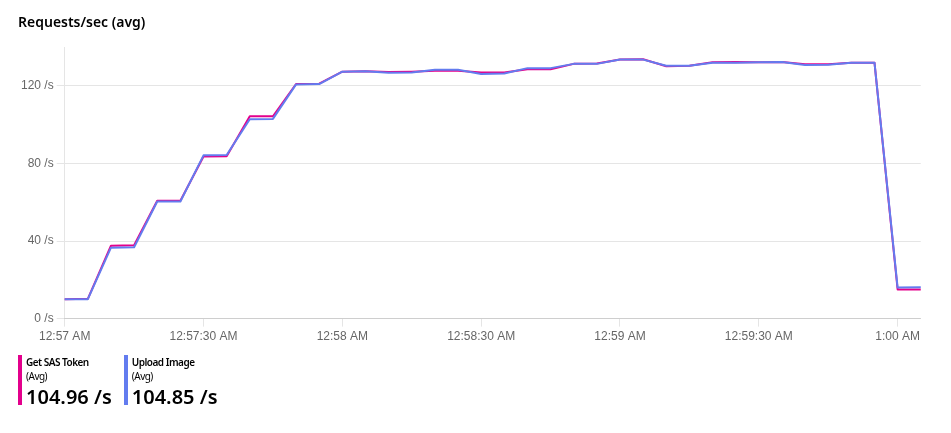
\includegraphics[width=\textwidth]{images_load.png}
        \caption{Carico delle richieste di caricamento delle immagini}
    \end{center}
\end{figure}
\clearpage
Il carico è stato impostato per aumentare gradualmente nei primi trenta secondi,
per poi continuare stabilmente fino a una durata massima di tre minuti.
L'immagine allegata ha una dimensione di quattro megabyte, 
in linea con la dimensione media di un'immagine effettuata da uno smartphone moderno.
In aggiunta alle metriche delle Azure Functions e del database,
si monitora anche Azure Storage Container.\\
\begin{figure}[htbp]
    \begin{center}
        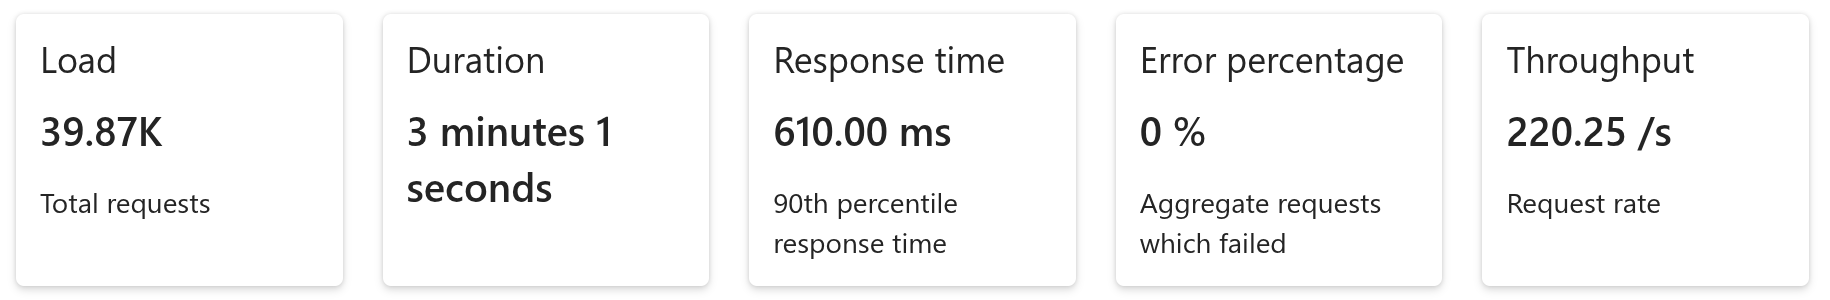
\includegraphics[width=\textwidth]{images_general.png}
        \caption{Risultati del caricamento delle immagini}
    \end{center}
\end{figure}
\\
Il test separa le due richieste, 
dando informazioni dettagliate sul comportamento di entrambe,
ma unendo infine i risultati.
Risultano quindi quasi quarantamila richieste effettuate in tre minuti,
equamente suddivise tra richieste alle Functions e richieste di caricamento.
Le richieste al secondo calcolate sono da considerarsi la somma delle due,
per cui, su un totale di duecentoventi richieste medie al secondo, 
il carico effettivamente ricevuto dallo Storage Container è di circa centodieci richieste al secondo.\\
\begin{figure}[htbp]
    \begin{center}
        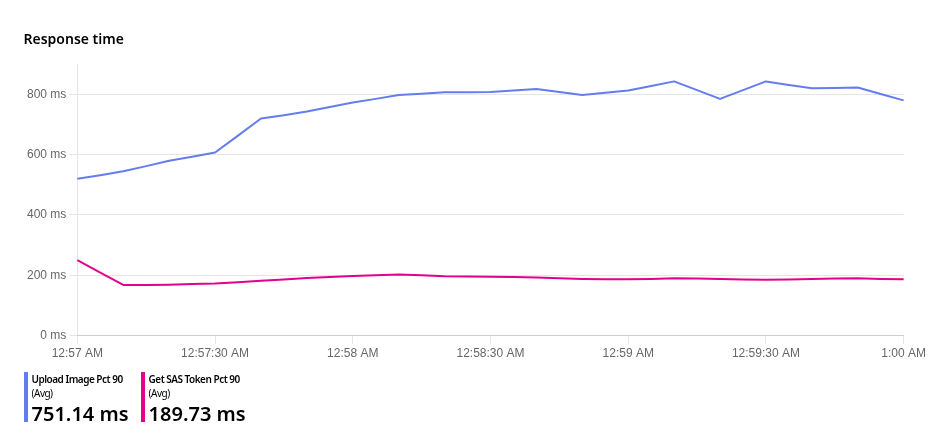
\includegraphics[width=\textwidth]{images_results.png}
        \caption{Tempi di risposta delle due richieste}
    \end{center}
\end{figure}
\\
La richiesta alle Azure Function risulta affidabile, 
mantenendo un tempo di risposta costante nonostante il carico, 
in linea con le richieste di scrittura sul database.
Questo indica che l'operazione di generazione del token 
non produce un impatto significativo sulle prestazioni e 
presenta le stesse caratteristiche di scalabilità del resto del sistema.
Analizzando invece il tempo di risposta del caricamento delle immagini,
più alto a causa della dimensione della richiesta,
ma ampiamente accettabile,
si nota però che varia in base al carico delle richieste.\\
\\
L'aumento del tempo di salvataggio delle immagini in linea con il carico comporta il pericolo 
che il sistema non risulti scalabile.
Per quanto sia positivo che il tempo di risposta non vari nonostante un periodo prolungato di richieste,
indicando una distribuzione delle risorse equilibrata e ben gestita,
la correlazione tra quantità di richieste e latenza del sistema
potrebbe risultare problematica se continuasse ad aumentare senza mai stabilizzarsi.
\begin{figure}[htbp]
    \begin{center}
        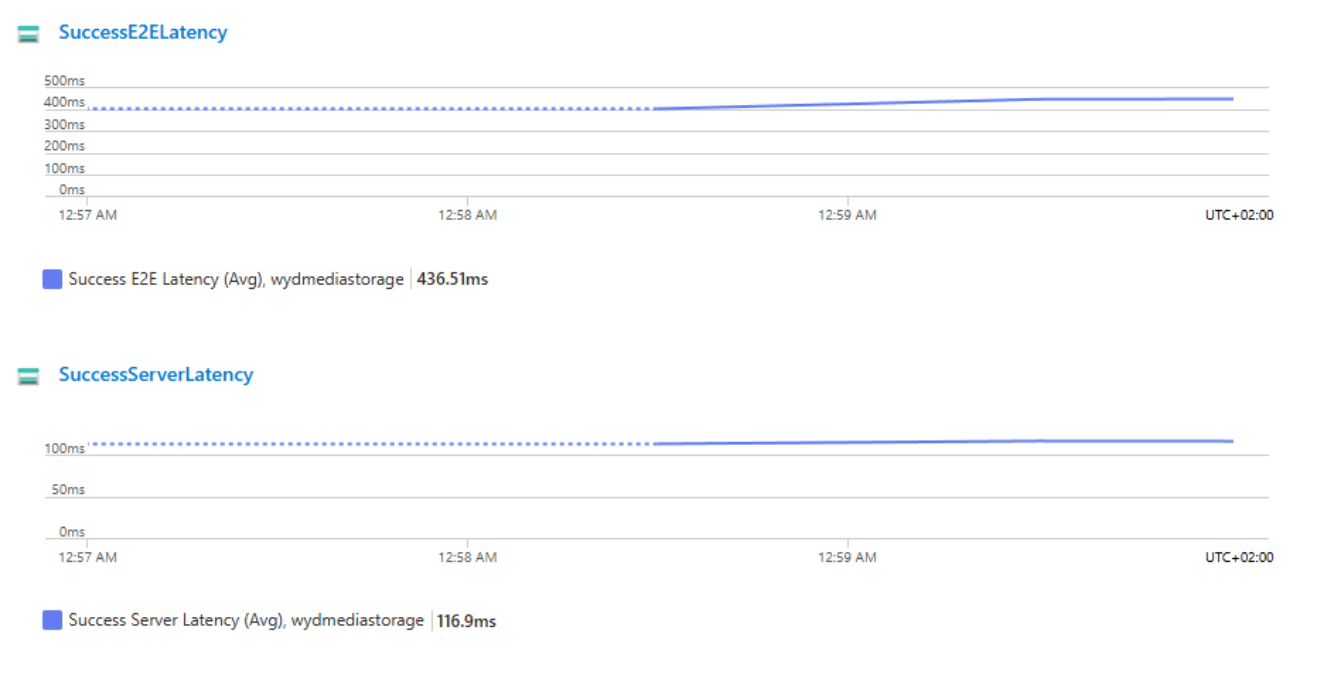
\includegraphics[width=\textwidth]{images_container_time.png}
        \caption{Dettaglio del tempo di risposta di Azure Storage Container}
    \end{center}
\end{figure}
\\
In generale, il caricamento delle immagini ha dato risultati positivi, 
garantendo la resilienza al caricamento simultaneo di file multimediali da parte di molti utenti in contemporanea, 
ma è necessario approfondire ulteriormente le prestazioni di caricamento delle immagini,
per verificare ulteriormente le proprietà di scalabilità fornite da Azure Storage Service.
\clearpage